
\section*{Question 3}

\begin{enumerate}[(a)]
    \item
    N=840\\
    \begin{figure}[h]
        \centering
        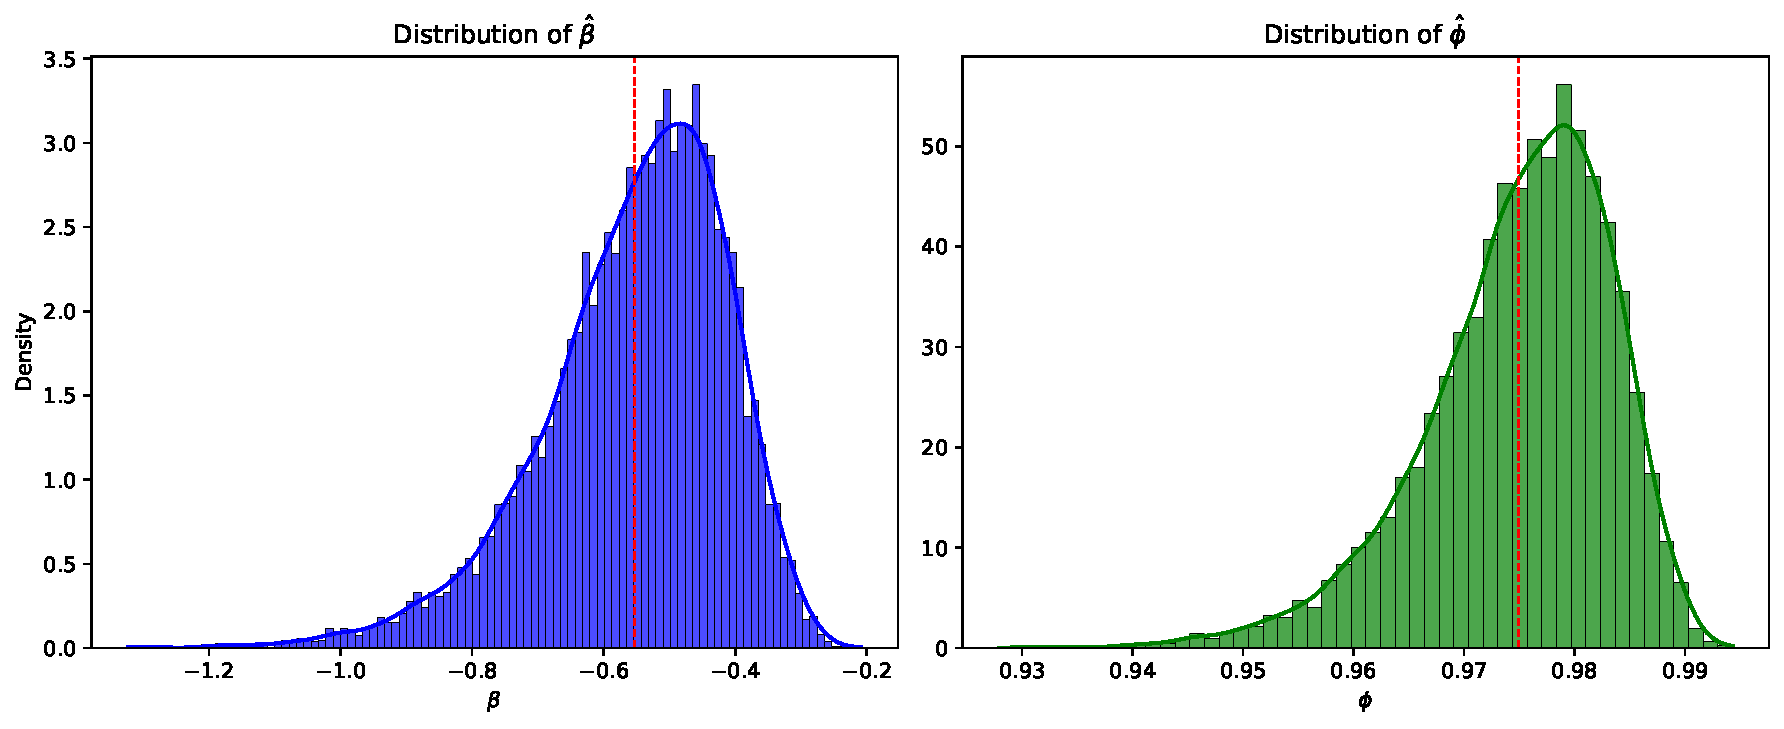
\includegraphics[width=0.9\linewidth]{Out/EX3-1.pdf}
        
    \end{figure}

  \item
    N=240\\
    \begin{figure}[h]
        \centering
        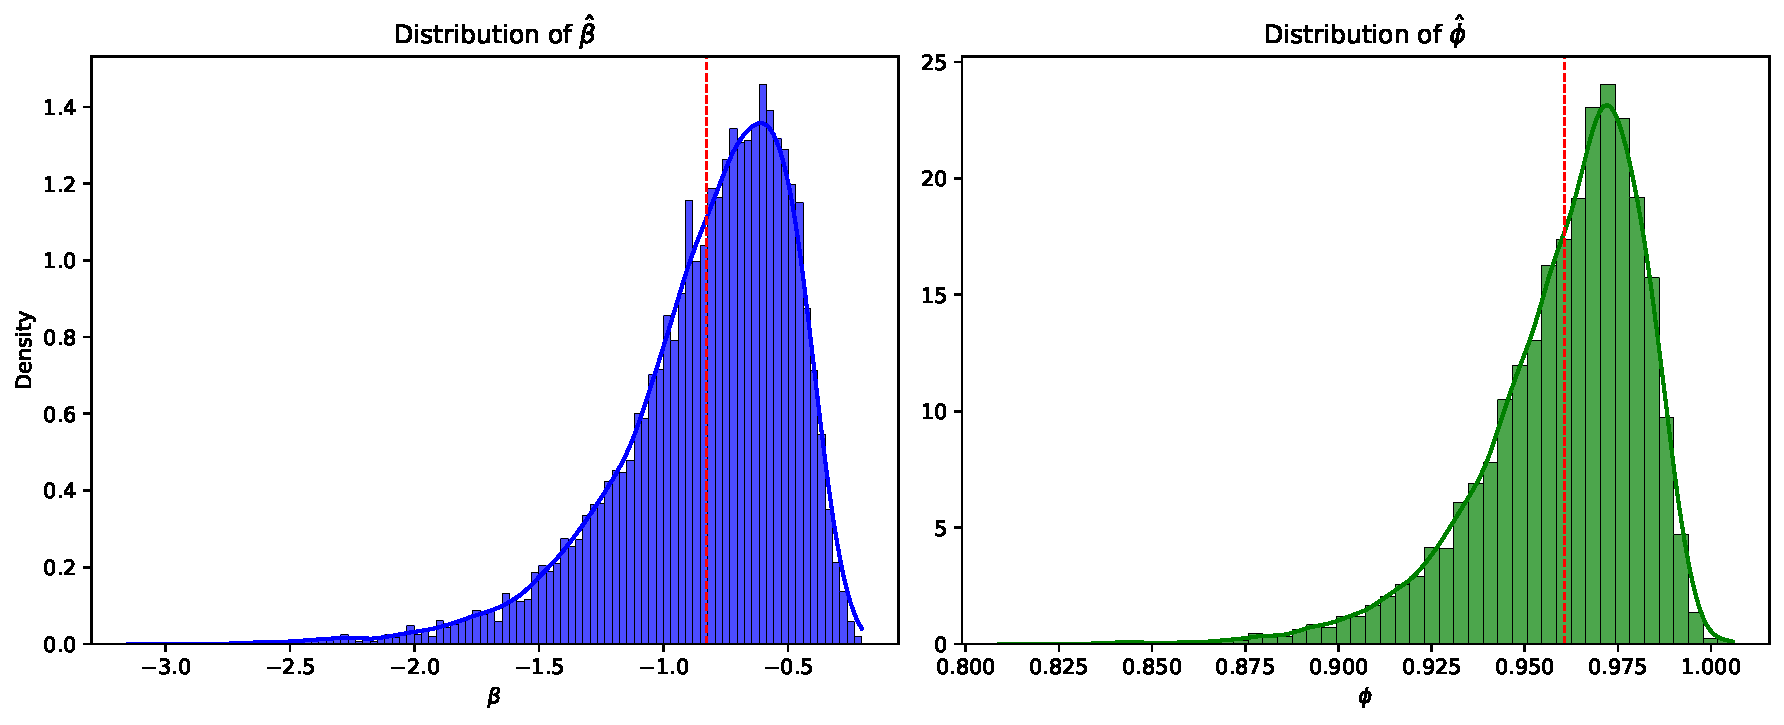
\includegraphics[width=0.9\linewidth]{Out/EX3-2.pdf}
        
    \end{figure}
Compared with the estimation with n=840, the estimation with n=240 is more biased, it's more skewed to the right side and away from the true value.



\begin{lstlisting}[language=Python, caption=Python code for simulation, label={lst:q1a}, escapechar=|, frame=single, basicstyle=\small, showstringspaces=false, captionpos=b, breaklines=true, showspaces=false, showtabs=false, keywordstyle=\color{blue}, commentstyle=\color{gray}]
    def simulate_and_estimate():
    # Initialize arrays to store parameter estimates
    beta_hat_array = np.zeros(n_replications)
    phi_hat_array = np.zeros(n_replications)

    for rep in range(n_replications):
        beta_hat_array[rep], phi_hat_array[rep] = simulate()

    return beta_hat_array, phi_hat_array

def simulate():
    r, x = generate_data()
        # Estimate parameters with OLS
    beta, phi = estimate_parameters(r, x)
    return beta, phi

def generate_data():
    # Simulate data
    # Correlation matrix
    corr_mat= np.array([[1.0, corr_uv],
                        [corr_uv, 1.0]])

    # Compute the (upper) Cholesky decomposition matrix
    upper_chol = cholesky(corr_mat)

    # Generate 3 series of normally distributed (Gaussian) numbers
    rnd = np.random.normal(0.0, 1.0, size=(n_obs, 2))

    # Finally, compute the inner product of upper_chol and rnd
    errors = rnd @ upper_chol
    u, v = errors[:, 0], errors[:, 1]
    # Scale errors
    u *= sigma_u
    v *= sigma_v 

    x = np.zeros(n_obs)
    r = np.zeros(n_obs)
    for t in range(1, n_obs):
        x[t] = theta + phi * x[t-1] + v[t]
        r[t] = alpha + beta * x[t-1] + u[t]
    return r, x

def estimate_parameters(r, x):
    # Estimate parameters with OLS
    model1 = sm.OLS(r, sm.add_constant(x))
    model2 = sm.OLS(x[1:], sm.add_constant(x[:-1]))
    results1 = model1.fit()
    results2 = model2.fit()
    # Store estimates
    beta_hat = results1.params[1]
    phi_hat = results2.params[1]
    return beta_hat, phi_hat
\end{lstlisting}
\item 
We rejected 0 times out of 10,000 when when assuming IID errors, 
suggesting that we reject the null hypothesis. 
However, we should be expecting high rejection rate since the real value of beta is 0.\\
This difference might be due to the fact that the errors are not independent.\\
 \textcolor{red}{New results [0.5051, 0.3815, 0.2619] for significance level 5\%, 1\%, 0.1\% respectively}

\begin{lstlisting}[language=Python, caption=Python code for new model, label={lst:q1a}, escapechar=|, frame=single, basicstyle=\small, showstringspaces=false, captionpos=b, breaklines=true, showspaces=false, showtabs=false, keywordstyle=\color{blue}, commentstyle=\color{gray}]
    def estimate_new_model(r,x):
    df = pd.DataFrame({'r':r,'x':x})
    df['12_month_return'] = df['r'].rolling(12).sum()
    # get the pvalue of the regression
    return sm.OLS(df['12_month_return'][11:].to_numpy(), sm.add_constant(df['x'][:-11]).to_numpy()).fit().pvalues[1]
def new_simulation():
    pvalue = np.zeros(n_replications)
    for rep in range(n_replications):
        r, x = generate_data()
        pvalue[rep] = estimate_new_model(r,x)
    return pvalue
    \end{lstlisting}

\item 
We rejected 9.77\% of the simulations out of 10,000 runs when using Newey-West standard errors, suggesting that there is autocorrelation present in the errors, and the standard errors are adjusted to account for this.\\
At the 10\% significant level, we would not reject the null hypothesis: H0: beta=0. 
\textcolor{red}{New results : [0.0913, 0.0326, 0.0067] for significance level 5\%, 1\%, 0.1\% respectively}

\begin{lstlisting}[language=Python, caption=Python code for new model with Newey-West, label={lst:q1a}, escapechar=|, frame=single, basicstyle=\small, showstringspaces=false, captionpos=b, breaklines=true, showspaces=false, showtabs=false, keywordstyle=\color{blue}, commentstyle=\color{gray}]
    def estimate_new_model_neweywest(r,x):
    df = pd.DataFrame({'r':r,'x':x})
    df['12_month_return'] = df['r'].rolling(12).sum()
    # get the pvalue of the regression
    return sm.OLS(df['12_month_return'][11:].to_numpy(), sm.add_constant(df['x'][:-11]).to_numpy()).fit(cov_type='HAC', cov_kwds={'maxlags': 11}).pvalues[1]
def new_simulation_neweywest():
    pvalue = np.zeros(n_replications)
    for rep in range(n_replications):
        r, x = generate_data()
        pvalue[rep] = estimate_new_model(r,x)
    return pvalue
    \end{lstlisting}
\end{enumerate}

